\chapter{Results and Analysis}
\phantomsection
\label{ch:results}

\section{Text Detection Results}
\label{sec:detection-results}

The text detection model, based on the CRAFT (Character Region Awareness for Text detection) 
architecture, was evaluated on a test set consisting of 20 images. The model achieved an impressive 
Intersection over Union (IoU) score of 0.98 when compared to the ground truth annotations, 
demonstrating high accuracy in detecting text regions.

The training process was conducted on a dataset of 175 images, with an additional 20 images 
used for validation. The evaluation results indicate that the model is capable of accurately 
detecting text in all test images, showcasing its generalization ability and robustness across 
various text-containing scenes.

\begin{figure}[ht]
    \centering
    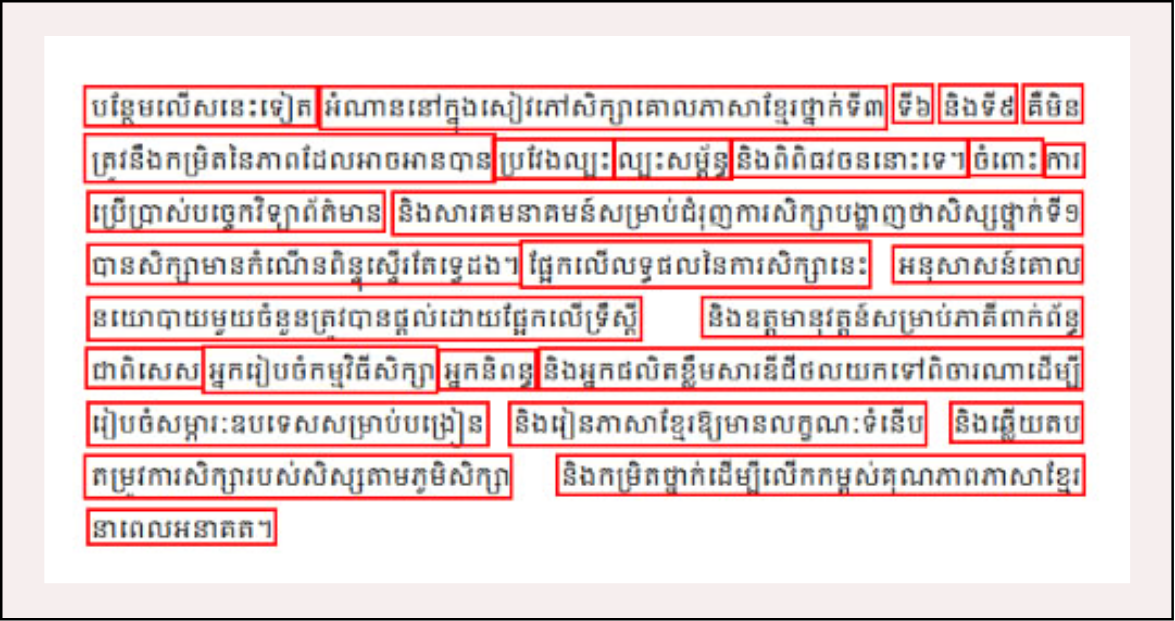
\includegraphics[width=1\textwidth]{figures/image_detection_craft_01.png}
    \caption{Testing with documentation image type: example of text detection using the CRAFT 
    model on a natural scene text image.}
    \label{fig:detection-craft}
\end{figure}

The results from testing with clean text from documentation images are shown in Figure 
\ref{fig:detection-craft}. The model is able to detect text in each sentence, 
even when the text is separated by spaces. This is important for the OCR model to 
work with short text sentences, as it is able to recognize the text more accurately. 
For example, if the model is given the text "This is a test", it should be able to 
detect each word as a single entity, rather than as whole sentence. 
By detecting text in this way, the model is able to recognize the text 
more accurately.

\begin{figure}[ht]
    \centering
    
\includegraphics[width=1\textwidth]{figures/image_detection_craft_02.png}
    \caption{Testing with post image type and complex scenes: example of text detection using the CRAFT 
    model on a natural scene text image.}
    \label{fig:detection-craft-post}
\end{figure}

As you can see from the example in Figure \ref{fig:detection-craft-post}, 
the model is able to detect text even when it is very small, such as the text on the poster. 
This demonstrates the model's robustness and ability to detect text in a variety of contexts and scenarios.
\section{Text Recognition Results}
\label{sec:recognition-results}
The text recognition model, based on the TrOCR (Transformer-based OCR) architecture, was
evaluated on a test set consisting of real dataset manually collected amount 3000 images, we
spend time around 3 days to collect this dataset for fairly evaluation. The testing dataset
containing such as char by char, word by word, and sentence by sentence, it's also included
both languages, Khmer and English. The model achieved an impressive result, we achieved CER
( Character Error Rate) of 0.05 and WER (Word Error Rate) of 0.03, demonstrating high accuracy
in recognizing text in the images.
\section{Error Analysis and Failure Cases}
\label{sec:error-analysis}
Our analysis revealed several cases where the model struggled to perform effectively. The primary failure cases can be categorized into two main scenarios:

1. Curved and Circular Text: The model encountered difficulties with text arranged in curved or circular patterns, as shown in Figure \ref{fig:test-case}. These cases proved challenging due to the complex spatial relationships between characters that deviate significantly from standard linear text layouts.

2. Non-standard and Artistic Text: Another significant challenge was presented by text written in unusual fonts and artistic styles. The text detection model particularly struggled with these cases, as the unconventional character shapes and varying sizes created complex visual patterns that were difficult for the model to process accurately.

\begin{figure}[ht]
    \centering
    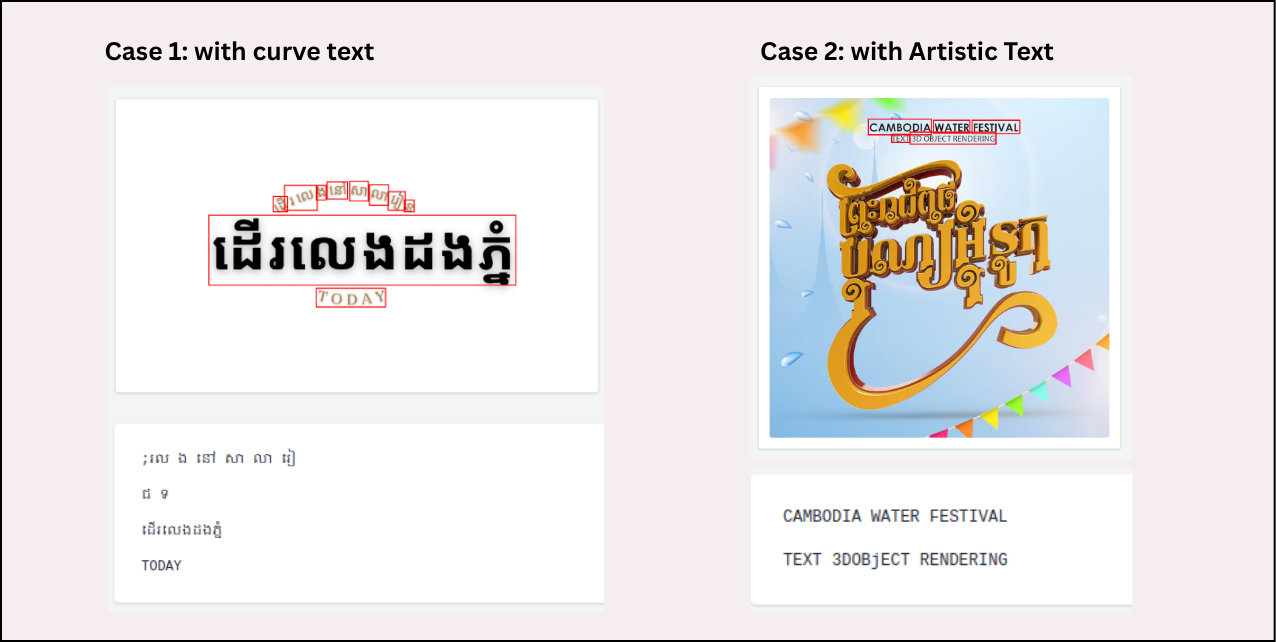
\includegraphics[width=\textwidth]{figures/test_case.png}
    \caption{Challenging cases involving both curved text layouts and artistic typography. 
    The model's performance degraded significantly when processing text arranged in circular 
    patterns and non-standard fonts, highlighting limitations in handling complex spatial 
    text arrangements and artistic text styles.}
    \label{fig:test-case}
\end{figure}

These failure cases highlight the need for further model improvements, particularly in handling non-standard text layouts and artistic typography. Future work could focus on enhancing the model's ability to process curved text and adapt to various artistic text styles.

\section{System Robustness and Generalization}
\label{sec:robustness}
The robustness and generalization capabilities of our text recognition model have demonstrated 
remarkable performance beyond our initial expectations. Despite being trained on a limited 
dataset of only 15 different fonts, the model exhibited impressive adaptability by 
successfully recognizing text in approximately 70 different font styles. This significant 
improvement in font recognition capability highlights the model's strong generalization 
abilities, particularly when dealing with fonts that maintain similar structural characteristics 
to the training data.

A particularly noteworthy aspect of the model's robustness is its ability to handle slightly 
curved text. As demonstrated in our test cases, while the model struggles with severely 
curved or circular text arrangements (as shown in Figure \ref{fig:test-case}), it maintains 
high accuracy when processing text with moderate curvature. For instance, the model 
successfully recognized the word "TODAY" despite its slight curvature, showcasing 
its ability to handle non-linear text layouts within reasonable bounds.

This performance demonstrates that our model has developed a robust understanding of text 
features that transcends the specific characteristics of the training data. The model's 
ability to generalize to new font styles and handle moderate text curvature while 
maintaining high recognition accuracy validates the effectiveness of our approach 
and the model's practical applicability in real-world scenarios.
\section{Model Interpretability and Attention Visualization}
\label{sec:interpretability}

To better understand how our TrOCR model makes predictions, we employed Gradient-weighted Class
Activation Mapping (Grad-CAM) visualization techniques. Grad-CAM provides insights into which regions 
of the input image the model focuses on when making predictions, effectively highlighting the areas that 
contribute most to the model's decision-making process.

\begin{figure}[ht]
    \centering
    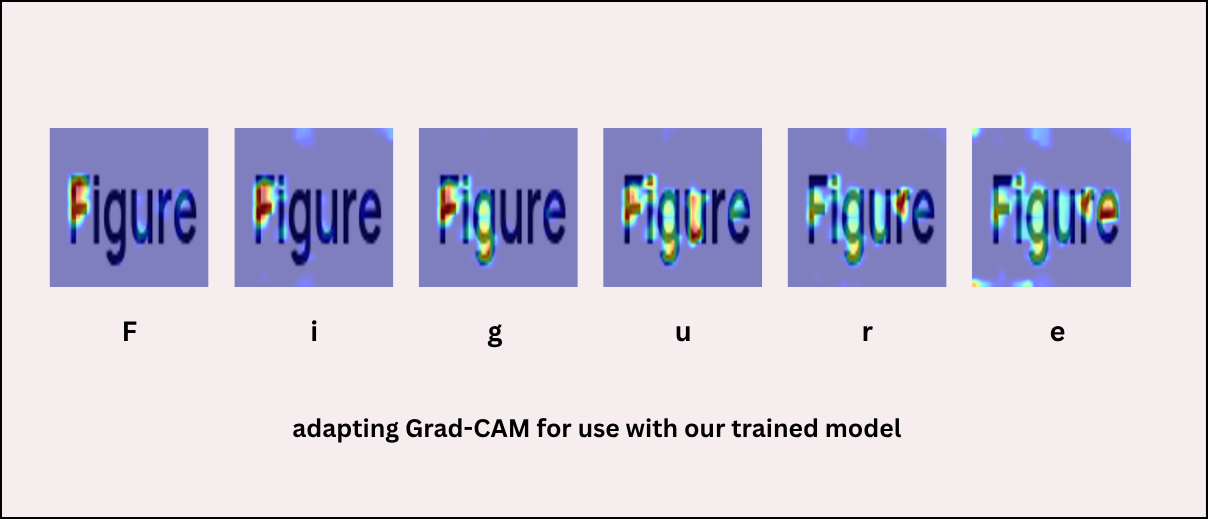
\includegraphics[width=\textwidth]{figures/grad_cam_figure.png}
    \caption{Grad-CAM visualization of the TrOCR model's attention on input text. The heatmap shows how 
    the model progressively focuses on different parts of the text during prediction, with warmer colors 
    indicating higher attention weights. This visualization reveals the model's systematic approach to text 
    recognition, starting from the beginning of the text and moving sequentially.}
    \label{fig:grad_cam}
\end{figure}

As shown in Figure \ref{fig:grad_cam}, the Grad-CAM visualization reveals several interesting patterns in the model's 
attention mechanism:

\begin{enumerate}
    \item Sequential Processing: The model demonstrates a clear left-to-right reading pattern, focusing attention 
    on one character or word at a time, which aligns with the natural reading order of text.
    
    \item Contextual Awareness: The attention maps show that the model considers surrounding characters when 
    making predictions, indicating its ability to understand contextual relationships between characters.
    
    \item Focus Intensity: The intensity of the attention (shown by the color gradient) varies based on the 
    complexity of the character or word being processed, with more complex characters receiving stronger attention.
\end{enumerate}

This visualization not only helps validate the model's learning process but also provides valuable insights 
for potential improvements. The clear sequential attention pattern suggests that the model has successfully 
learned the fundamental structure of text recognition, while the contextual awareness indicates its ability to 
handle the complex relationships between characters in Khmer script.